\documentclass{article}

\usepackage{physics}
\usepackage{amsmath}
\usepackage[margin=0.8in]{geometry}
\usepackage{graphicx}
\usepackage{bm}
\let\vec\bm

\title{Transfer Report}
\author{Fergus Barratt}

\begin{document}
\maketitle
\section{Introduction}
The effective use of quantum technology requires the systems we build to be isolated from the environment.
In general this can only be achieved approximately.
In this project, we investigate the role of the world at large in three different ways
\begin{enumerate}
    \item In gate-based quantum computation, the threshold theorem says that any local environmental influence can be overcome by error correction.
          No such theorem exists for adiabatic quantum computation. 
          We introduce tools from classical statistical mechanics to characterise the failure of adiabatic quantum computation.
    \item We introduce a useful connection between different ways of treating the environment.
    \item Classical systems exhibit dynamical chaos - an exponential sensitivity to initial conditions. 
          In quantum systems classical chaos is impossible.
          What role does the standard tool for characterising dynamical chaos - the lyapunov spectrum - play in the quantum case?
          We build on some earlier work in this area, and compare to standard tools for evaluating quantum chaos.
\end{enumerate}
%
%%
\section{Failure of Adiabatic Quantum Computation}\label{sec:failure}
%%
\subsection{Introduction}
%
Adiabatic Quantum Computation (AQC) is an alternative (equivalent~\cite{Aharonov2004}) paradigm of quantum computation.
We prepare the ground state of some easily accessed Hamiltonian.
If we tune the parameters in the hamiltonian sufficiently slowly, then by the adiabatic theorem~\cite{born1928adiabatic} the system will remain in the ground state of the time varying hamiltonian.
By transforming the state in this way we can perform a quantum computation.

Whilst the effect of the environment on gate-based quantum computation is well understood, the same is not true about AQC.
In particular, for gate-based QC we have threshold theorems that suggest that if we have access to sufficiently many qubits we can overcome the effects of local noise. 
In the following, we introduce methods popularised in the study of classical glasses to characterise failure in AQC.
\subsection{Dynamical Phase Transitions}
Phase transitions are conventionally understood by a free energy, which becomes discontinuous as a function of some system parameter. 
One standard example is found in the classical Ising model in two dimensions, in which we can distinguish a paramagnetic from a ferromagnetic phase by a discontinuity in the free energy as a function of temperature.
Each phase is characterised by the value of some order parameter, in this case the magnetisation.
A more rigorous understanding of this formalism can be achieved by using large deviation theory. 
The partition function 
\begin{equation}
    \mathcal{Z}_N(\beta) = \ev{e^{-\beta H}}
\end{equation}
is the moment generating function (MGF) of the energy in the probability distribution over microstates.
The free energy 
\begin{equation}
    f(\beta) = \lim_{N\rightarrow\infty} \frac{1}{N} \mathcal{Z}_N(\beta)
\end{equation}
is the \emph{scaled cumulant generating function} (sCGF) associated with this probability distribution.

AQC is a dynamical process, and the failure of AQC is a dynamical transition - computational trajectories which support sufficient entanglement succeed, and those that don't, fail. 
If this failure can be characterised by an order parameter, it must be dynamical, that is must depend on a whole trajectory. 
In studies of the glass transition~\cite{Garrahan2007}, a formalism was introduced for characterising just this kind of transition.
We define the \emph{dynamical partition function}
\begin{equation}
    \mathcal{Z}_t(s) = \ev{e^{-sQ}}\label{eq:mgf}
\end{equation}
where $Q = \int^t \dd{t'} I(t')$ is some time-extensive (in this case time-integrated) observable, and the average is taken over an ensemble of trajectories.
$s$ is a generating parameter, of which more later.
We can thus define:
\begin{equation}
    \varphi(s) = \lim_{t\rightarrow\infty} \frac{1}{t} \ln\mathcal{Z}_t(s), \label{eq:cgf}
\end{equation}
the \emph{dynamical free energy}.
Dynamical phase transitions are discontinuities in the dynamical free energy, and seperate phases characterised by a dynamical order parameter.
%
\subsubsection{Bias}
%
In the static case, the free energy depends on the inverse temperature $\beta$, which has a sensible physical meaning. 
In the dynamical case the interpretation of the parameter $s$ is not clear. 
We can understand $\beta$ as a bias on the microcanonical ensemble, making certain states more or less probable, depending on their energy.
In the same way $s$ makes certain trajectories more or less probable, depending on the value of $Q$.

In AQC, it is the environment that biases trajectories - for stronger dissipation, trajectories with less entanglement are more likely. 
We will show that these biasing effects are one and the same - that is, environmental bias can be understood as a bias on an ensemble of quantum trajectories. 
%
\subsubsection{Quantum Mechanics}
%
There are subtleties associated with understanding eqs.~\ref{eq:mgf} and~\ref{eq:cgf} for quantum systems. 
In particular, given that measurements in quantum mechanics are commonly understood as single shot operations, how can the exponent of eq.~\ref{eq:mgf} be understood?
The answer is provided by the full counting statistics~\cite{Nazarov2001}.
In Ref~\cite{Hickey2013} the $s$-biased states are introduced
\begin{equation}
    \ket{s} = \flatfrac{e^{i(H-is\hat{I})t} \ket{\Omega}}{\norm{e^{i(H-is\hat{I})t} \ket{\Omega}}}\label{eq:bias}
\end{equation}
in terms of which 
\begin{equation}
    \varphi(s) = -\ev{k}{s}/s\label{eq:dyn}
\end{equation}
\subsection{The Failure of Adiabatic Quantum Computation as a Dynamical Phase Transition}
We apply the above ideas in a simple model of AQC, and show the equivalence of trajectory bias and environmental influence.
%
\subsubsection{Two Spin model}
%
The simplest model in which we can consider the effect of entanglement as a resource is two coupled spins-half. 
We consider a Heisenberg Hamiltonian
\begin{equation}
    H = \vec{\sigma}_1\cdot\vec{\sigma}_2 -h(t) \left(\sigma_1^z-\sigma_2^z\right)\label{eq:hamiltonian}
\end{equation}
where a staggered longitudinal field is scanned from $-\infty$ (where the ground state is $\ket{\uparrow\downarrow}$) to $\infty$ (where the ground state is $\ket{\downarrow\uparrow}$).
The system undergoes an Adiabatic Quantum Computation, where entanglement must be sustained - since the ground state at $h=0$ is the maximally entangled singlet. 
Since the dynamics at $h=0$ determine the success of the computation, we consider the dynamics of the Hamiltonian in the presence of noise. 

{\it Parametrisation: } We parametrise the Hilbert Space in the following way
\begin{equation}
    \ket{\psi} = n_1 \ket{\vec{l}_1, \vec{l}_2} + n_2 \ket{-\vec{l}_1, -\vec{l}_2}\label{eq:parametrisation}
\end{equation}
Where $\vec{l}_1$ denotes a spin coherent state, and $\braket{\vec{l_i}}{-\vec{l}_i} = 0$.
We can consider a Bloch vector $\vec{n} = \begin{pmatrix} n_1^* & n_2^* \end{pmatrix}\vec{\sigma} \begin{pmatrix} n_1 \\ n_2 \end{pmatrix}$, such that a point in hilbert space can be specifed with two sets of local degrees of freedom ($\ev{\sigma^i_j} = n_z l_i^j$) and one set of nonlocal degrees of freedom $\vec{n}$.
In particular, the Schr\"odinger equation in this parametrisation becomes the classical Hamiltonian equations of motion if $n_z=1$ is constrained.

{\it Zero Magnetization: } With the initial state $\ket{\uparrow \downarrow}$, the local degrees of freedom $\vec{l}_1 = \vec{z}$ and $\vec{l_2} = -\vec{z}$ undergo no dynamics. 
All that remains is the dynamics of $\vec{n}$.
The computation above becomes an adiabatic rotation between the poles of the $\vec{n}$ sphere.

{\it Aside - SU(2) Dynamics: } In the zero magnetization subspace, the state lies on the Bloch sphere. 
One might suspect that it is possible to find some set of operators $\vec{n}$ that span the subspace we are interested in - in fact this is the case
\begin{equation}
    \vec{\hat{n}} = \begin{pmatrix} (\sigma_1^+\sigma_2^-+\sigma_1^-\sigma_2^+) \\
                                  -i(\sigma_1^+\sigma_2^--\sigma_1^-\sigma_2^+) \\
                                    (\sigma_1^z-\sigma_2^z) 
                    \end{pmatrix}
\end{equation}
where $\vec{n} = \ev{\vec{\hat{n}}}$, and the operators $\hat{n}_i$ satisfy the spin commutation relations in general, and the pauli matrix anticommutation relations when projected onto the magnetization zero subspace.
In this language, the Hamiltonian is $H = J/2(\hat{n}_x -\hat{n}_z^2)+h(t)\hat{n}_z$.
Projected onto zero magnetization subspace, the nonlinearity vanishes, and the dynamics become obvious
\begin{equation}
    \dot{\vec{n}} = (J \hat{x}  - h(t) \hat{z})\cross \vec{n}
\end{equation}

{\it Noise: } Motivated by experiments on flux qubits, where environmental influence has different origins in different directions, we add local anisotropic noises $\eta_i^z\sigma_i^z$ to the Hamiltonian Eq.~\ref{eq:hamiltonian}. 
Since $\sigma_1^z+\sigma_2^z$ commutes with the Hamiltonian, we can consider just $H+\tilde{\eta}(\sigma_1^z-\sigma_2^z)$, where $\tilde{\eta} = \eta_1^z-\eta_2^z, \overline{\tilde{\eta}} = 0, \overline{\tilde{\eta}(t)\tilde{\eta}(t')} = \gamma\delta(t-t')$.

{\it Density Matrix Dynamics} The equations of motion for the vector $\vec{n}$, when averaged over the noise, are
\begin{equation}
    \dot{\vec{\bar{n}}} = (J \hat{x} - h(t) \hat{z}) \cross \vec{\bar{n}} - \gamma \hat{z} \cross(\vec{\bar{n}} \cross \hat{z})\label{eq:total}
\end{equation}
in which we can isolate an angular part
\begin{equation}
    \dot{\vec{n}} = (J \hat{x} - h(t) \hat{z}) \cross \vec{\bar{n}} - \gamma n_z \vec{n} \cross(\hat{z} \cross\vec{n})\label{eq:ang}
\end{equation}
and a radial part
\begin{equation}
    \dot{r} = - \gamma (1-n_z^2) r\label{eq:rad}
\end{equation}
since $\bar{\vec{n}} = r \vec{n}$ no longer lies on the surface of the Bloch sphere.
%
\subsubsection{Dynamical Phase Transition}
We can turn Eq.~\ref{eq:bias} into a Schr\"odinger type equation by expanding to first order in t
\begin{equation}
    i\partial_t\ket{s} = (H-is/2(I-\ev{I}))\ket{s}.\label{eq:sch}
\end{equation}
Biased dynamics are \emph{a priori} a new kind of dynamics.
We would expect that some sort of entanglement bias might be most clearly connected with dissipation.
However, entanglement is not a simple observable and we can't directly bias with it. 
We observe nonetheless that $\hat{n}_z$ is connected to several measures of entanglement: $\ev{n_z} = \abs{n_1}^2-\abs{n_2}^2$ is the difference between the Schmidt coefficients of the system, and the variance $\ev{(n_z-\ev{n_z})^2}$ is the concurrence $C = 2(1-\tr(\rho^2))$, a lower bound to the Von Neumann Entanglement Entropy. 

If we replace $I$ in Eq.~\ref{eq:sch} with $(n_z-\ev{n_z})^2$, a (time dependent) operator, whose expectation is the concurrence, we derive the following equation
\begin{equation}
    \dot{\vec{n}} = (J \hat{x} - h(t) \hat{z}) \cross \vec{\bar{n}} - s n_z \vec{n} \cross(\hat{z} \cross\vec{n})\label{eq:bias_dyn}
\end{equation}
which is identical to Eq.~\ref{eq:ang}! Anisotropic dissipation is identical to bias with an entanglement measure.

{\it Dynamical Free Energy: } Biasing with the variance is strange. 
Still, we expect that features in the corresponding dynamial free energy should be represented in the dynamical free energy corresponding to the operator itself, that is, if we calculate Eq.~\ref{eq:dyn} with $\hat{n}_z$ bias (which can be done by diagonalising $H-is\hat{n}_z$), any discontinuities we find must be represented in Eq.~\ref{eq:bias_dyn} and thus in Eq.~\ref{eq:total}.
We show in Fig.~\ref{fig:dyn} this is indeed the case. 
The dynamical free energy is non-analytic at $\flatfrac{s}{J} = 2$. 
Correspondingly, as $\gamma/J$ becomes greater than two, trajectories that start below the equator never reach the upper hemisphere - the Hamiltonian at $h=0$ does not dynamically connect the lower and upper hemispheres, and thus the quantum computation must fail. 
We conclude that the dynamical phase transition and the failure of adiabatic quantum computation are one and the same. 

\begin{figure}[h]
    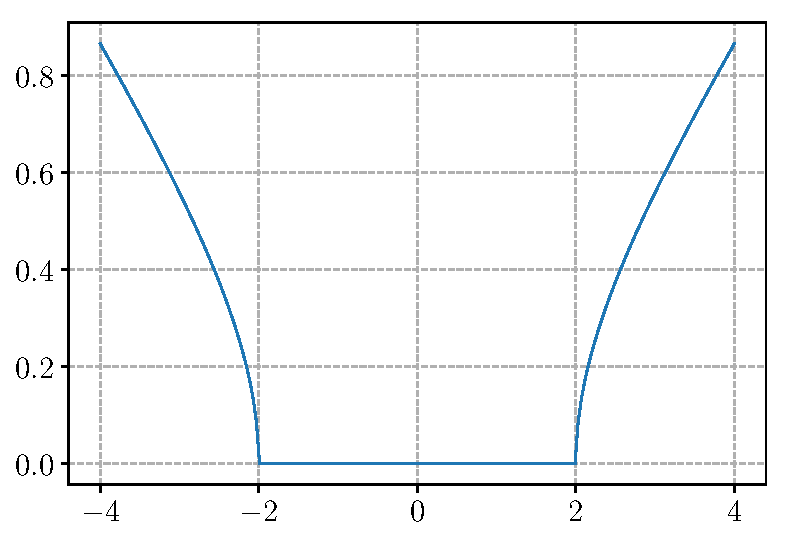
\includegraphics[width=0.49\linewidth]{bare_transition.pdf}
    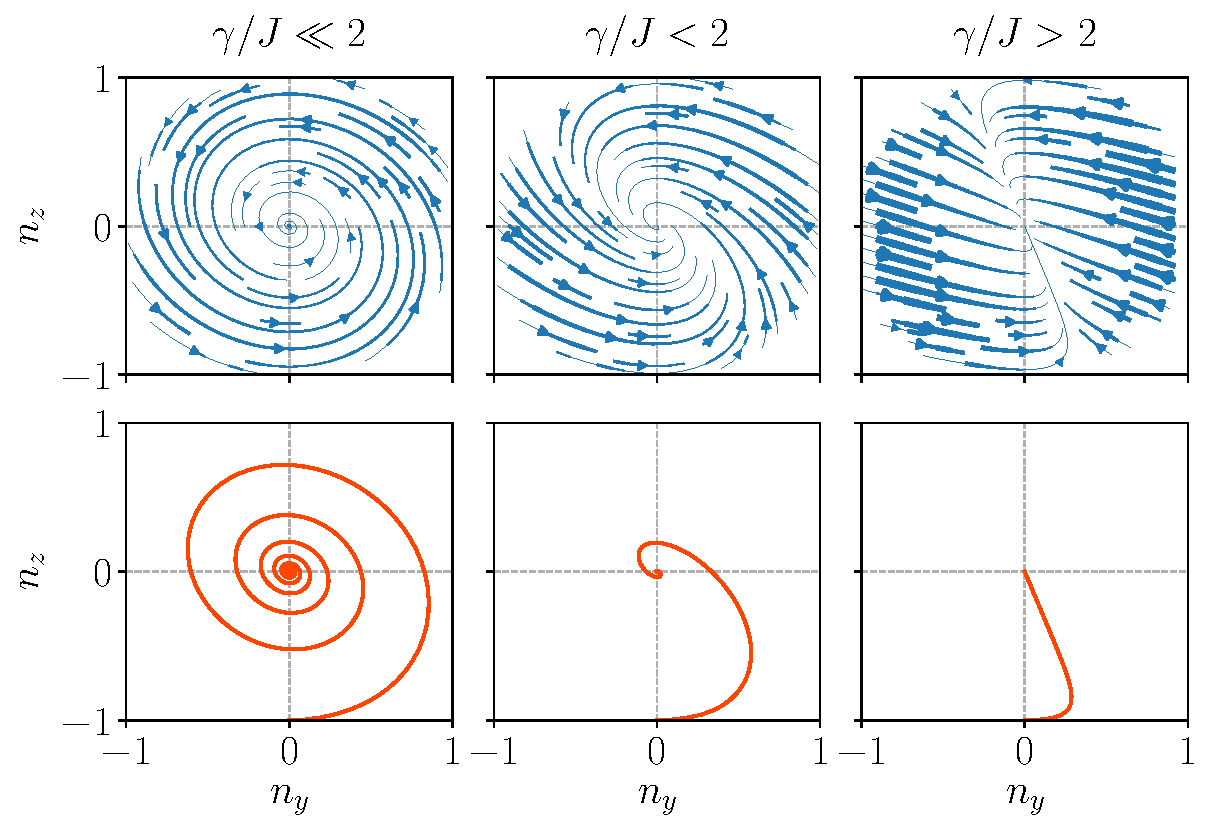
\includegraphics[width=0.5\linewidth]{diss.pdf}
    \caption{Dynamical Free energy}\label{fig:dyn}
\end{figure}

%
\section{Keldysh Field Theory \& the Lindblad Equation}\label{sec:open}
%
\subsection{Introduction}
The Lindblad equation has become the standard tool for treating Markovian open quantum systems. 
Keldysh Field Theory allows us to write field theoretic descriptions of open quantum systems. 
In general the two represent distinct ways of describing open quantum systems - nevertheless, for consistency they must each be derivable from the other. 
In the following we derive the Lindblad Equation from a Keldysh Field Theory.
\subsection{Action}
The Keldysh action for linear coupling via operators $\hat{\mathcal{L}}_\mu$ to a local, quadratic bath is
\begin{equation}
    S = \int_t^{t'}\left[ \dd{s} L[\vec{\varphi}_s] +  \sum_{\mu, \gamma} \left(\alpha_{\mu, \gamma}\vec{\mathcal{L}}^\dagger_\mu \hat{\sigma}_3 \vec{\varphi}_r^\gamma + \alpha_{\mu, \gamma}^* \vec{\varphi}^{\gamma\dagger}_r \hat{\sigma}_3 \vec{\mathcal{L}}_\mu \right) + \sum_\gamma \vec{\varphi}^{\gamma\dagger}_r(s) \mathcal{G}_{\gamma}^{-1}(s) \vec{\varphi}_r^\gamma(s)\right].
\end{equation}
where the correlators are given by
\begin{equation}
    \mathcal{G}_{\gamma}(t, t') 
    \equiv 
    \begin{bmatrix}
        g_{\gamma}^{++}(t, t') & g_{\gamma}^{+-}(t, t') \\
        g_{\gamma}^{-+}(t, t') & g_{\gamma}^{--}(t, t') 
    \end{bmatrix}.
\end{equation}
Performing a gaussian functional integral over the bath fields yields
\begin{equation}
    S = \int_t^{t'} \dd{s}\left[L[\vec{\varphi}_s] +  \sum_\mu \int_t^{t'}\dd{s'} \vec{\mathcal{L}}_\mu(s)^\dagger \mathcal{G}_\mu'(s, s') \vec{\mathcal{L}}_\mu(s')\right],\nonumber\label{eq:action}
\end{equation}
where the correlators are now
\begin{equation}
    \mathcal{G}'_\mu(t, t') \equiv \left[\sum_{\gamma}|\alpha_{\gamma, \mu}|^2 \begin{bmatrix} -g_\gamma^{++}(t, t') & g_\gamma^{+-}(t, t') \\ g_\gamma^{-+}(t, t') & -g_\gamma^{--}(t, t')\end{bmatrix} \right].
\end{equation}
The system action eq.~\ref{eq:action} is the result of the following approximations
\begin{enumerate}
        \item Quadratic Bath: We assume the bath can be well approximated by a local, quadratic action.
        \item Linear coupling: We assume that the coupling to the bath can be described by a (generic) linear coupling to (potentially nonlinear and nonhermitian) system operators $\hat{\mathcal{L}}_\mu$.
        \item Born approximation: We assume no entanglement is generated between system and bath.
\end{enumerate}
\subsection{Keldysh Rotation}
Performing a Keldysh rotation on the action eq.~\ref{eq:action}, and decoupling the term quadratic in $\mathcal{L}_\mu^q$ with a Hubbard-Stratonovich transformation
\begin{align}
    S &= \int_t^{t'} \dd{s}L[\vec{\varphi}_s]\\
    &+  \sum_\mu \int_t^{t'}\dd{s'}\Big[\left[g_R(s, s') \bar{\mathcal{L}}_\mu^c(s)\mathcal{L}^q_\mu(s')+\bar{g}_R(s', s) \mathcal{L}_\mu^c(s')\bar{\mathcal{L}}^q_\mu(s)\right] + \bar{\eta}_\mu(s) \mathcal{L}_\mu^q + \eta_\mu(s) \bar{\mathcal{L}}_\mu^q + \bar{\eta}_\mu(s) \left[g_K(s, s')\right]^{-1}\eta_\mu(s') \Big]\nonumber
\end{align}
\subsubsection{Exact saddle point}
The 
\begin{align}
    S &= \int_t^{t'} \dd{s} \bra{\varphi_q(s)} \Big[i\partial_t - H-\sum_\mu\left(\bar{\eta}_\mu(s)\mathcal{L}_\mu + \eta_\mu(s)\mathcal{L}^\dagger_\mu\right)\nonumber \\
    &\qquad\qquad\qquad\quad~~ + \int_t^{t'} \dd{s'} \left(g_R(s', s)\left\{\ev{\mathcal{L}^\dagger}^c_{s'} +\ev{\mathcal{L}^\dagger}^q_{s'}\right\}\mathcal{L}_\mu + \bar{g}_R(s', s) \left\{\ev{\mathcal{L}}^c_{s'}+\ev{\mathcal{L}}^q_{s'}\right\}\mathcal{L}_\mu^\dagger\right)\Big]\ket{\varphi_c(s)} \\
    &+ c.c.\\
    &+ \bar{\eta}_\mu(s) \left[g_K(s, s')\right]^{-1}\eta_\mu(s') \Big]\nonumber
\end{align}
\subsubsection{Quantum fields approximation}
If we make the following approximation
\begin{equation}
    \mel{\varphi^q}{\mathcal{L}_\mu}{\varphi^q} = 0
\end{equation}
this is the (now exact, since the target manifold is the whole hilbert space) saddle point
\begin{equation}
    i\partial_t \ket{\psi(t)} =\left[H(t) + \sum_\mu \left(\bar{\eta}_\mu(t) \hat{\mathcal{L}}_\mu(t) + \eta_\mu(t)\hat{\mathcal{L}}^\dagger_\mu \right) + \int^t\dd{t'} \Gamma(t-t') \partial_t \bar{\ev{\mathcal{L}_\mu}} \mathcal{L}_\mu(t) + \int^t\dd{t'} \bar{\Gamma}(t-t') \partial_t \ev{\mathcal{L}_\mu}\mathcal{L}^\dagger_\mu(t)\right]\ket{\psi(t)}\nonumber
\end{equation}
where we have also assumed $g_R(s', s) = \Gamma(s-s')$. 
The saddle point is a stochastic, nonlinear Schr\"odinger equations, that depends on the whole past history of the system. 
The noise correlations are set by the Keldysh correlator, and the memory of the noise by the retarded and advanced correlators. 

\subsection{The Lindblad Equation}
In the Lindblad limit $\Gamma(t-t') = 0$ and $\ev{\bar{\eta}_\mu(t)\eta_{\mu'}(t')} = \delta_{\mu\mu'}\delta(t-t')$, so
\begin{equation}
    i\partial_t \ket{\psi(t)} =\left[H(t) + \sum_\mu \left(\bar{\eta}_\mu(t) \hat{\mathcal{L}}_\mu(t) + \eta_\mu(t)\hat{\mathcal{L}}^\dagger_\mu \right)\right]\ket{\psi(t)}\nonumber
\end{equation}
From which with stochastic calculus one can derive the quantum master equation. 
Alternatively, assuming local correlators from the outset with the following form,
\begin{align}
    \mathcal{G}'_\mu(t, t') = J_\mu\delta(t-t') \begin{bmatrix} -\frac{1}{2} & 0 \\ 1 & -\frac{1}{2}\end{bmatrix}
\end{align}
we can proceed with a slight modification of the derivation of Feynman and Hibbs~\cite{Feynman},
We use that the density matrix propagates as
\begin{equation}
    \rho_{\vec{z}'}(t') = \int \dd{\vec{z}} \left[\int_{\vec{z}}^{\vec{z'}} \mathcal{D}[\vec{\varphi}]e^{iS'[\vec{z}]} \right]\rho_{\vec{z}}(t)\label{eq:prop}.
\end{equation}
For infinitesimal $\varepsilon = t-t'$, one can use the following approximation for the kernel
\begin{align}
    &\int_{\vec{z}}^{\vec{z}'} \mathcal{D}[\vec{\varphi}]\exp{i\int_t^{t+\varepsilon} L(\vec{\varphi}, \dot{\vec{\varphi}})}\nonumber \\
    &\qquad\qquad= \frac{1}{A} \exp{i\varepsilon L\left[\frac{(\vec{z}+\vec{z}')}{2}, \frac{(\vec{z}-\vec{z})}{\varepsilon}\right]},\label{eq:approx}
\end{align}
where $L$ is the Lagrangian and $A$ is a normalisation constant defined by the condition that the kernel be normalised to $1$.
In the absence of a bath, the lagrangian in the Keldysh action will be of the form $L[\vec{z}] = L_c[z^+]-L_c[z^-]$, where $L_c$ is the standard classical action (i.e.\ from the Feynman path integral).
We illustrate the emergence of the master equation for a single particle system in one dimension, but the higher dimensional case follows with minor modifications.
Starting from the single particle action,
\begin{equation}
    L_c[x] = \frac{m\dot{x}^2}{2} - V\left(x\right),
\end{equation}
with the approximation of eq.~\ref{eq:approx} and the reservoir terms present, the kernel for short times for propagation from $\vec{z} = (x, y)$ to $\vec{z}' = (x', y')$ is
\begin{align}
    K &= \frac{1}{A} \exp{i\frac{m}{2}\frac{\left({x}'-{x}\right)^2-\left({y}'-{y}\right)^2}{\varepsilon}}\\
    &\times \exp{i\varepsilon \left[V\left({x}'+{x}\right)-V\left({y}'+{y}\right) + \sum_\mu \mathcal{D}_\mu(\vec{x}+\vec{x}')\right]}\nonumber
\end{align}
The denominator of the first exponential factor causes rapid phase oscillations that strongly supress large deviations in final position.
We take $\vec{z} = \vec{z}' - \vec{\eta}$, where $\eta^\pm  \sim \mathcal{O}(\sqrt{\varepsilon})$, and expand the kernel in eq.~\ref{eq:prop} to order $\varepsilon$. 
\begin{align}
    \rho_{\vec{z}'}&(t+\varepsilon) = \int \dd{\vec{\eta}}\frac{1}{A} \exp{i\frac{m}{2}\frac{\vec{\eta}^T\hat{\sigma}_3\vec{\eta}}{\varepsilon}}\\
    &\times \exp{i\varepsilon \left[V\left({x'}\right)-V\left({y'}\right) + \sum_\mu \mathcal{D}_\mu(\vec{x'})\right]}\rho_{\vec{z}'-\vec{\eta}}(t).\nonumber
\end{align}
expanding both sides to order $\varepsilon$, performing a number of gaussian integrals, and converting equations of motion for matrix elements to equations for operators (bearing in mind the operator ordering implied by the time ordering), we have
\begin{equation}
    \partial_t \hat{\rho}(t) = -i \comm{H}{\hat{\rho}(t)} + \sum_\mu J_\mu\left( \mathcal{L}_\mu\hat{\rho}(t)\mathcal{L}_\mu^\dagger - \frac{1}{2} \acomm{\mathcal{L}_\mu^\dagger\mathcal{L}_\mu}{\hat{\rho}(t)}\right)\nonumber
\end{equation}
the Lindblad equations.
%%
\section{Lyapunov Spectra in Matrix Product State Simulations}\label{sec:chaos}
%%
%
\subsection{Introduction}
%
According to the classical definition, chaos is precluded in quantum systems by the unitarity of the Schr\"odinger equation.
Quantum evolution does show signatures of chaos however, and the role of classical chaos in i.e.\ thermalization is performed in other ways.
In this section we build on the work of Ref.~\cite{Andrew}, in which a connection is made between classical chaotic dynamics and thermalisation via Lyapunov spectra extracted in several semiclassical limits.
%
\subsubsection{Lyapunov Exponents and the Lyapunov Spectrum}
%
The Lyapunov exponents characterise the rate of growth of infinitesimal perturbations to an initial condition.
%
\subsubsection{Matrix Product States and the Time Dependent Variational Principle}
%
Matrix Product States (hereinafter MPS) provide a convenient parametrisation of wavefunctions in 1 dimension.
%
\subsubsection{Entanglement Growth and the Out of Time Ordered Correlator}
%
Thermalization in classical systems is driven by classical chaos. 
In quantum systems, it is believed that the growth of entanglement serves to scramble nonlocal information and thermalise local operators. 
It should be possible to connect the two approaches, and in particular there should be a connection between the rate of growth of entanglement and the Lyapunov spectrum. 
We verified numerically the following conjecture
\begin{equation}
    \dot{S}_E = \frac{S_{KS}(D(t))}{D(t)^2}
\end{equation}
for the rate of growth of the von Neumann entanglement entropy at time $t$.
$S_{KS}$ is the Kolmogorov-Sinai Entropy: the sum of the positive Lyapunov Exponents. 
$D(t)$ is the smallest bond dimension that captures the dynamics exactly at time $t$.
%
\subsubsection{Spin Waves}
%
The TDVP is the saddle point of a Matrix Product state field theory.
We can expand around this saddle point, and include quadratic fluctuations.
For $D=1$, this is a spin wave expansion.
In general, after expanding the Hamiltonian to quadratic order in the Holstein-Primakoff bosonic operators at time $t$, 
\begin{equation}
    H(t) = \begin{pmatrix} \vec{a}^\dagger & \vec{a} \end{pmatrix}
           \begin{pmatrix} A(t) & B(t) \\ B^*(t) & A^*(t) \end{pmatrix}
           \begin{pmatrix} \vec{a} \\ \vec{a}^\dagger \end{pmatrix}
\end{equation}
where the vector should be understood as having both site indices and operator indices, and $A, B$ are 
\begin{align}
    A_{ij}(t) &= \mel{\partial_i\psi}{H}{\partial_j\psi}\\
    B_{ij}(t) &= \mel{\partial_i\partial_j\psi}{H}{\psi}.
\end{align}
Such a hamiltonian can be diagonalised at each time by a bogoliubov transformation~\cite{colpa}
\begin{equation}
    H = \sum_r \omega_r \gamma_r^\dagger \gamma_r
\end{equation}
where
\begin{equation}
    \begin{pmatrix} \vec{\gamma}\\ \vec{\gamma}^\dagger \end{pmatrix}
    = \begin{pmatrix} P & Q \\ Q^* & P^* \end{pmatrix}
    \begin{pmatrix} \vec{a} \\ \vec{a}^\dagger \end{pmatrix}.
\end{equation}
In general $P$ and $Q$ must be determined by an involved procedure~\cite{colpa}.
For the case $B=0$ - i.e.\ the absence of anomalous terms, we have $Q=0$. 
Otherwise $Q \neq 0$.
Since the hamiltonian is diagonal in the Bogoliubov operators, we have also their time dependence, and the time dependence of the $a_i$
\begin{equation}
    \vec{a}(t) = F(t) \vec{a} + G(t) \vec{a}^\dagger
\end{equation}
$F$ and $G$ are matrices in the site space. 
For nearest neighbour hamiltonians without anomalous terms: 
\begin{align}
    F_{ij}(t)&= \frac{1}{N} \sum_k e^{-i(\omega_k t - k(j-j'))}\\
    G &= 0
\end{align}
note that $F$ is unitary for all time - in fact this is generically the case. 
It leads to $(a^\dagger a)(t) = a^\dagger a$. 
In general however $(a^\dagger a)(t) = (a^\dagger a)(0)+(aa^\dagger)(0)+F^*(t)G(t)(a^\dagger a^\dagger)(0) + G^*(t)F(t)(a a)(0)$.

Writing the spin operators in the HP basis, with $L = F+G, R=F-G$,
\begin{align}
    \vec{S}_x(t) &= L^R(t)\vec{S}_x + R^I(t)\vec{S}_y\\
    \vec{S}_y(t) &= L^I(t)\vec{S}_x + R^R(t)\vec{S}_y\\
\end{align}
At first order $n-$site operators spread to sums of $n-$site operators, but higher order expansions of the HP operators lead to operator spreading.
%
\subsection{Out of Time Ordered Correlator}
%
\begin{align}
    C(t) &= -\ev{\comm{S_i^z(0)}{l^j_\alpha S_j^\alpha(t)}^2}\\
         &= -\ev{\left[(l^i_x(t) L^R_{ii}(t)+ l^i_y(t) L^I_{ii}(t)) S_i^y(0)-(l_i^x(t)R^I_{ii}(t) + l^i_y(t) R^R_{ii}(t))S_i^y(0))\right]^2}\\
         &= -\ev{p^2(t){S_i^x}^2+q^2(t){S_i^y}^2 + p(t)q(t)\acomm{S_i^x}{S_i^y}}
\end{align}
$p(t) = l^i_x(t) L^R_{ii}(t)+ l^i_y(t) L^I_{ii}(t)$, $q(t) =-(l_i^x(t)R^I_{ii}(t) + l^i_y(t) R^R_{ii}(t))$

\bibliographystyle{unsrt}
\bibliography{bibliography}
\end{document}
